%!TEX root = ../report.tex

\chapter{Context}
\label{chap:chap3}

\section*{}

The primal objective of this dissertation, as referred in chapter \ref{chap:intro}, is to develop one or more software modules that will improve Spotify Users' music discovery and recommendation experience using visual tools to represent the music artists' relations and Spotify's streaming service to provide high quality music stream.


The initial proposal was to develop a module that implements, at least, one of the following features:

\begin{enumerate}
  \item \label{item:obj1} Integrate Spotify's music stream into RAMA's website
  \item \label{item:obj2} Integrate information from the Spotify user into RAMA
  \item \label{item:obj3} Improve RAMA's features and design
  \item \label{item:obj4} Integrate the RAMA concept into a Spotify Application
  \item \label{item:obj5} Integrate RAMA's playlist generation into a Spotify Application
  \item \label{item:obj6} Integrate some of the above mentioned modules into a Mobile Application
\end{enumerate}

The first three functionalities (\ref{item:obj1}, \ref{item:obj2} and \ref{item:obj3}) focus on improving RAMA using Spotify's API, i.e. to integrate Spotify into RAMA.
Whereas \ref{item:obj4} and \ref{item:obj5} aim to integrate RAMA's concept into Spotify, through a Spotify Application (it would work as a plugin to Spotify's Desktop Client).
The last one (\ref{item:obj6}) would focus on implementing the previous functionalities into an Android, iOS or Windows Phone Application.

This chapter aims to analyse every single drawback of each possibility that affects the choice of which modules do develop, and on which environments it fits better: Spotify Application, Mobile Application, or RAMA improvements.

At first, Spotify's development environment will be introduced \ref{sec:spotify} in order to assess which tools are available for developers.
Next, the available tools will be evaluated in order to determine which ones fit the proposed modules to be developed, mostly, through experiments. 

By the end of this chapter the modules developed should be clearly stated, as well as which tools were used in the prototype.

The prototype should pursue the objective of contributing to an improved user experience when discovering new music taking advantage of visual tools that implement RAMA's concept.

\section{Introducing Spotify} % (fold)
\label{sec:spotify}

  Spotify is a Music Streaming Service that allows the user, through an Internet connection, to listen to any track (if available in the user's country) in Spotify's catalogue.
  The service was launched in 2008 with a native desktop client application.

  % clients available: desktop client, webplayer and mobile apps
  Now, the service has several types of clients available to the users: desktop client, webplayer and mobile applications.

  \begin{description}
    \item[\textbf{Desktop Client}] Desktop version of Spotify, with Windows and Mac versions (and also a Linux preview version).
    \item[\textbf{Webplayer}] Web version of Spotify. This was released in 2013, and spotify still advises the use of the native applications for a better user experience.
    \item[\textbf{Mobile Applications}] The mobile applications are available for Android and iOS devices.
  \end{description}

  \subsection{Development Tools} % (fold)
  \label{sub:devtools}
  
    Spotify provides a set of tools\footnote{http://developer.spotify.com/technologies} to develop Third-party Applications (websites, native applications and mobile applications) and Spotify Applications (that run inside Spotify's Desktop Client).
    There are five tools, each with different purposes.

    \subsubsection{Spotify Apps} % (fold)
    \label{ssub:spotify_apps}
      Spotify Applications\footnote{https://developer.spotify.com/technologies/apps} are a special case in the whole set of tools provided by Spotify.
      These applications are designed to run \emph{inside} the Desktop Client.
      Hence, its development is also inside the same environment.

      Spotify users can run and install applications from the store called "App Finder".
      All the applications are free.

      In \ref{fig:spotify_apps} on can see the interface of the desktop client.
      In this case, the discovery mode's interface.

      \begin{figure}
        \begin{center}
          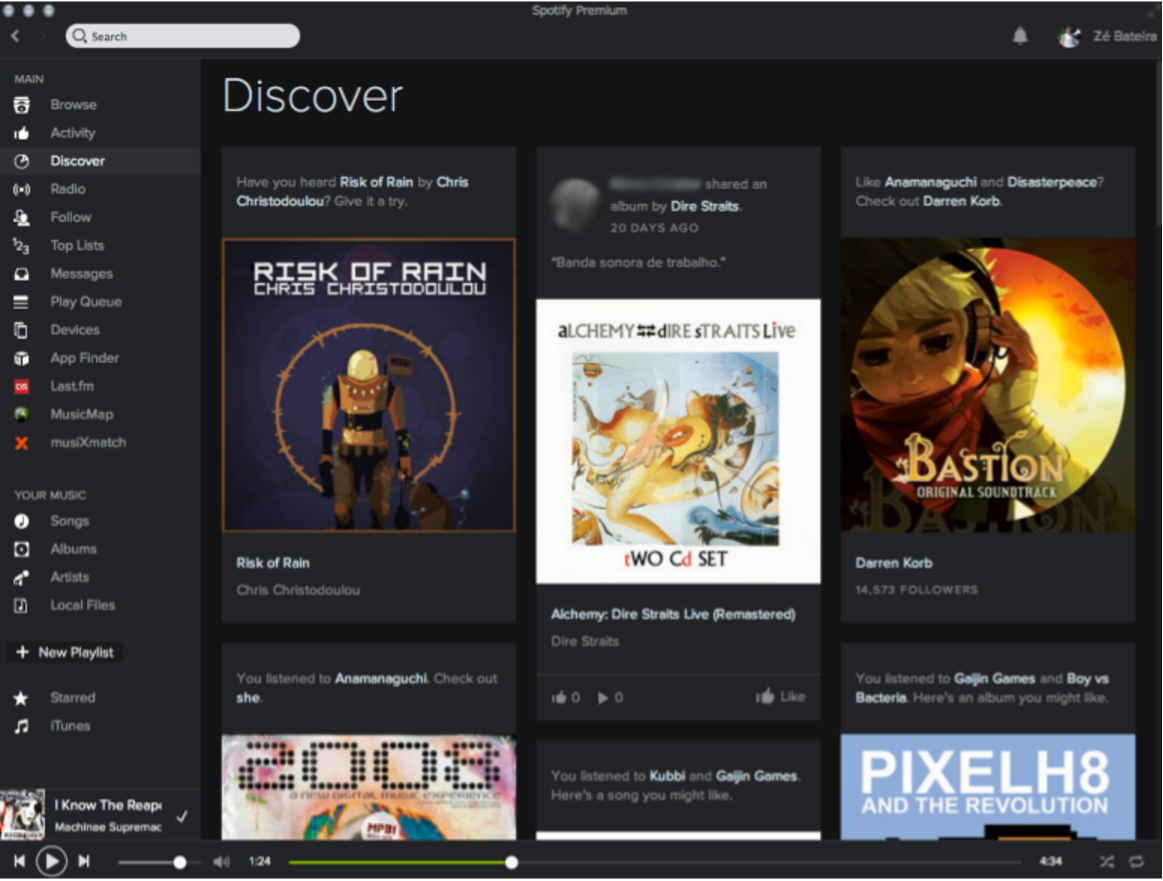
\includegraphics[width=\textwidth]{spotify_discovery.mode.pdf}
        \end{center}
        \caption{Spotify: desktop client's discovery mode interface.}
        \label{fig:spotify_apps}
      \end{figure}

      On the left side, in the menu, bellow the "App Finder" item, appears all the applications the user as installed from the store.

      In \ref{fig:spotify_apps2} the official Last.fm application is opened.
      Note how the space filled by the applications are always the same.

      \begin{figure}
        \begin{center}
          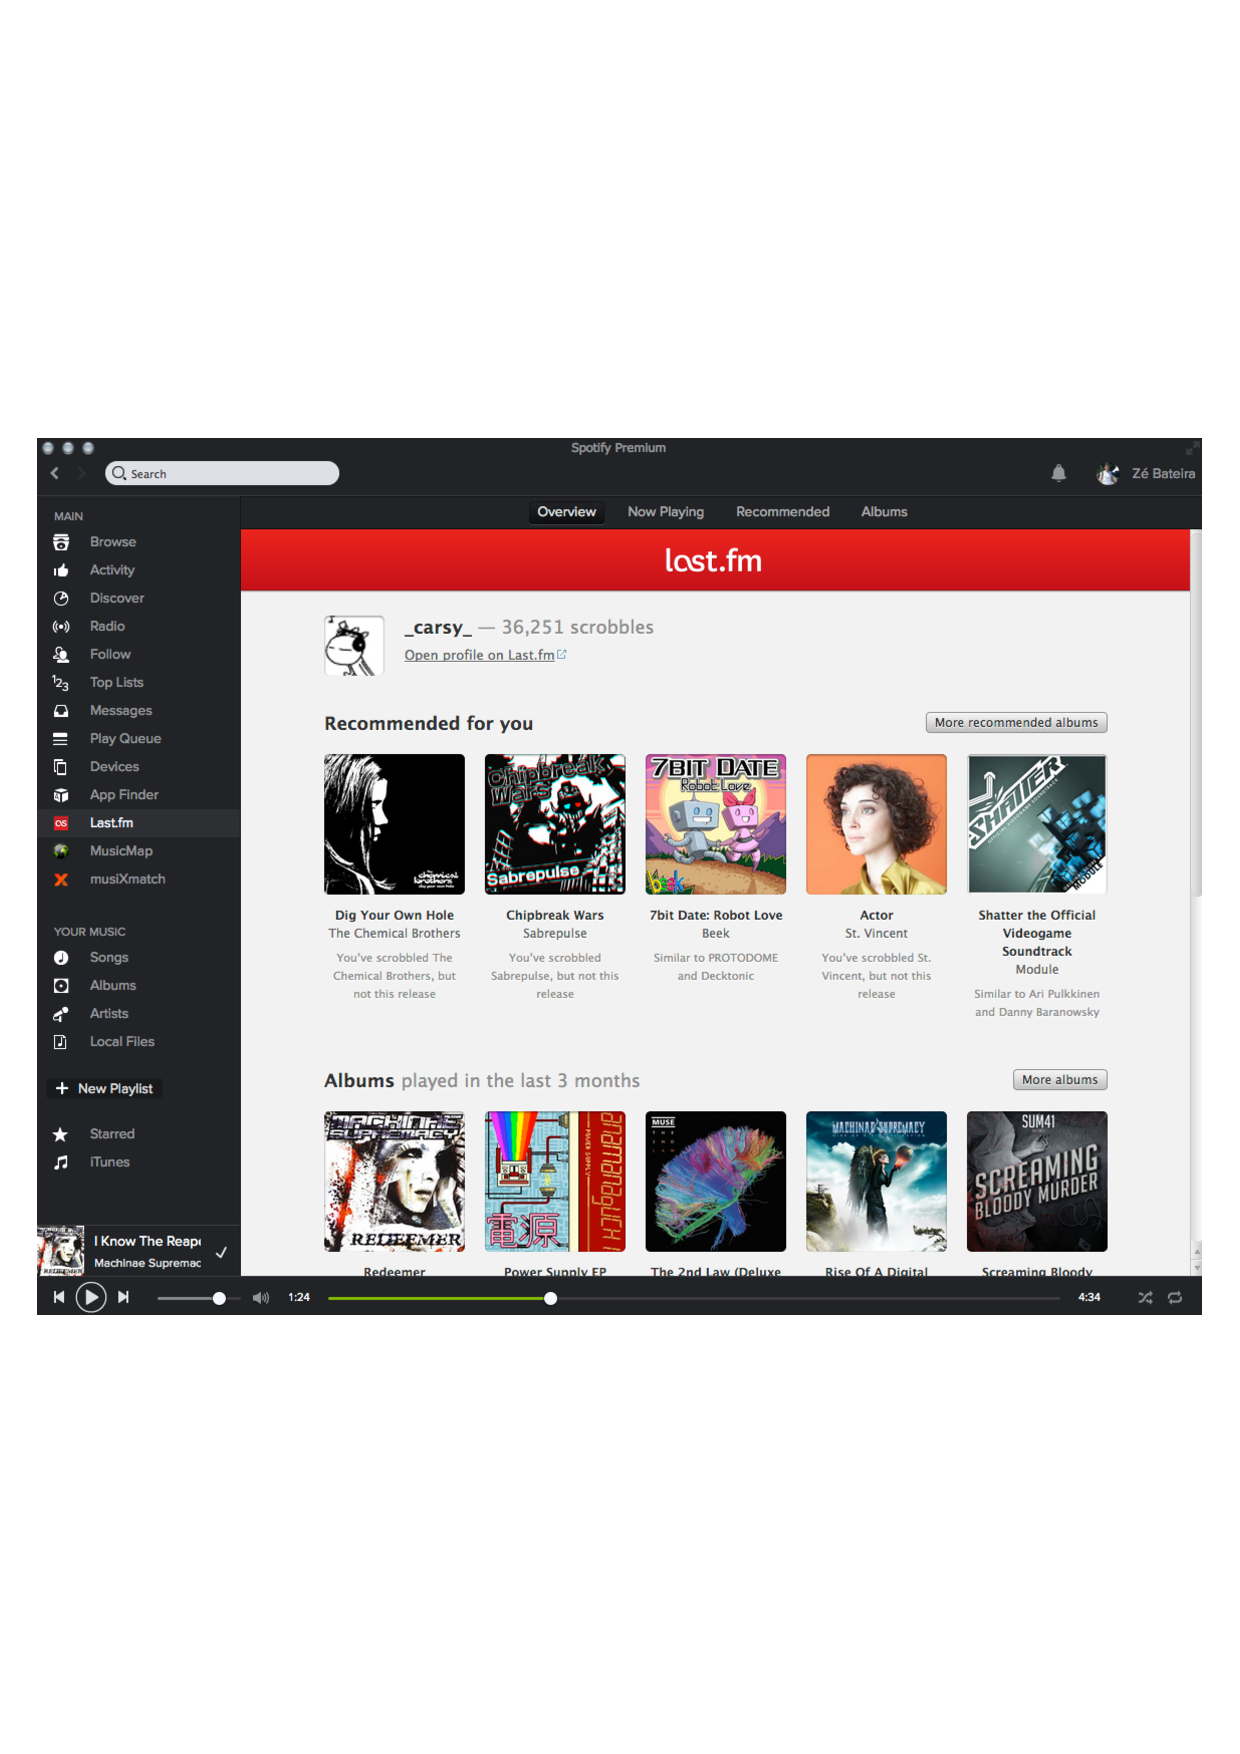
\includegraphics[width=\textwidth]{spotify_apps.pdf}
        \end{center}
        \caption{Spotify: Last.fm's Spotify Application opened.}
        \label{fig:spotify_apps2}
      \end{figure}

      The Applications' runtime environment is one of a browser-based.
      More specifically, powered by the Chromium Embedded Framework\footnote{https://code.google.com/p/chromiumembedded}.
      This means that the code to develop a Spotify Application follows the same principles as a web application: HTML, CSS and Javascript.

      Spotify developed two Frameworks\footnote{https://developer.spotify.com/technologies/apps/reference} to help developers create these applications: the API 1.x Framework\footnote{https://developer.spotify.com/docs/apps/api/1.0/} and the Views Framework\footnote{https://developer.spotify.com/docs/apps/views/1.0/}.

      The first one provides an interface to use object models, access metadata, control the player, among others.
      The second offers support for web components like buttons, lists, tabs, among others.

      In order to develop the proposed modules \ref{item:obj4} and \ref{item:obj5}, these are the most appropriate tools.

    % subsubsection spotify_apps (end)


    \subsubsection{Spotify Widgets} % (fold)
    \label{ssub:spotify_widgets}

      Spotify Widgets\footnote{https://developer.spotify.com/technologies/widgets} are small web components that can be embedded in external websites.
      Spotify provides two components: \emph{Play Button} (\ref{fig:spotify_play_button}) and a \emph{Follow Button} (\ref{fig:spotify_follow_button})

      \begin{figure}
        \begin{center}
          
\includegraphics{spotify_play_button.pdf}
        \end{center}
        \caption{Spotify: \emph{Play Button}.}
        \label{fig:spotify_play_button}
      \end{figure}

      \begin{figure}
        \begin{center}
          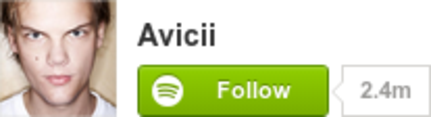
\includegraphics{spotify_follow_button.pdf}
        \end{center}
        \caption{Spotify: \emph{Follow Button} Allows the user to follow the music artist.}
        \label{fig:spotify_follow_button}
      \end{figure}

      However, there are some limitations.
      In Spotify, only logged in users can use the service (listen to tracks, etc).
      This also applies to these widgets - Even if they are in an external application, only Spotify users can interact with them.

      This limitation does make sense in the case of the \emph{Follow Button}, but the \emph{Play Button} becomes useless to non-spotify users.

      In truth, these widgets are nothing but an hyperlink to a Spotify Client (Web Player or Desktop).
      With the Play Button, the stream of tracks always played inside Spotify's environment, and not on external applications.

      To embed a widget, it is only required to copy-paste Html code into the website, where appropriate:

      \lstinputlisting[language=HTML,caption={Html code to embed the \emph{Play Button}}, style=htmlcssjs]{snippets/play_button.html}

      These widgets are useful to develop the proposed modules \ref{item:obj1} and \ref{item:obj3}.

    % subsubsection spotify_widgets (end)

    \subsubsection{Libspotify SDK} % (fold)
    \label{ssub:libspotify_sdk}

      Libspotify SDK\footnote{https://developer.spotify.com/technologies/libspotify} is an API that allows for third-party applications to include Spotify's services into them.
      However, not without some limitations to the users of these applications.
      The users are limited depending on the type of Spotify Subscription that they have signed up to.

      There are three different types of subscriptions, but the important part to retain, is the difference between being a Free Subscription Spotify User, and a Paid Subscription Spotify User (premium and unlimited subscriptions).
      As mentioned before (\ref{ssub:spotify_widgets}), only Spotify users can interact with the widgets.
      That also applies to third-party applications that are using Libspotify SDK, which allow, for example, the user to login with their Spotify account.
      But in this case, not only they need to be Spotify users, they also need to have signed up to a paid Spotify subscription.
      And not only do the users need to pay to use the Spotify-powered application, but the developers as well.

      This is a very restrictive environment, although Libspotify SDK comes in many different flavours\footnote{https://developer.spotify.com/technologies/libspotify/\#libspotify-downloads}.

      This tool would be used to develop modules \ref{item:obj1}, \ref{item:obj2} and \ref{item:obj6}.
      

    % subsubsection libspotify_sdk (end)


    \subsubsection{Metadata API} % (fold)
    \label{ssub:metadata_api}

      The \emph{Metadata API}\footnote{https://developer.spotify.com/technologies/web-api} allows for applications to retrieve information from Spotify's music catalogue: tracks, albums, artists, playlists, and so on.

      Requests to the database are done through HTTP and are of two types: \emph{search}\footnote{https://developer.spotify.com/technologies/web-api/search} e \emph{lookup}\footnote{https://developer.spotify.com/technologies/web-api/lookup}.

      To request detailed information of, e.g., an artist, the URI (used as the unique identifier) of that artist is required. Such ID is of the form:

      \url{spotify:artist:<artist_id>}, where \emph{artist\_id} is the unique identifier of the artist.

      Example:

      \url{spotify:artist:65nZq8l5VZRG4X445F5kmN}, is the ID for the artist "Mariza". \\

      There's also ID's for albums:

      \url{spotify:album:5d1LpIPmTTrvPltx26TlEU} (album "Fado Tradicional" from "Mariza") \\

       and for tracks:

       \url{spotify:track:2vqYasauhDLVjTt7CGWK6y} (track "Fado Vianinha" of the previous album) \\

      These URI schemes are compliant with Rosetta Stone's ID spaces\footnote{http://developer.echonest.com/docs/v4\#project-rosetta-stone}.

      First, to get this URI, one needs to search the database.

      \begin{description}
        \item[\emph{Search}] \hfill

          The base \emph{URL}:

          \url{http://ws.spotify.com/search/1/album}, to search for albums.

          For artists, \emph{artist}, for tracks, \emph{track}. \\

          Examples:

          \url{http://ws.spotify.com/search/1/album?q=foo} \\
          \url{http://ws.spotify.com/search/1/artist.json?q=red+hot} \\

          The request response, by default, is formatted in \emph{XML}, although, as the second example demonstrates, \emph{JSON} is also supported.

          Given the following query: \\
          \url{http://ws.spotify.com/search/1/artist.json?q=camane}

          The server responds with:

          \lstinputlisting[caption={Results ordered by "popularity"}, style=htmlcssjs]{snippets/search_camane.json}

        \item[\emph{Lookup}] \hfill \\

          When the URI is known, one can finally lookup detailed information about a database item. With the following \emph{query}: \\
          \url{http://ws.spotify.com/lookup/1/.json?uri=spotify:artist:3MLPFTe4BrpEV2eOVG0gLK}

          The server responds with:

          \lstinputlisting[caption={\emph{lookup} of the artist "Camané"}, style=htmlcssjs]{snippets/lookup_camane.json}

      \end{description}

      This API is very useful to all the six proposed modules.

    % subsubsection metadata_api (end)

    \subsubsection{iOS SDK (beta)} % (fold)
    \label{ssub:ios_sdk}
    
    The iOS SDK supports iOS Application developers. Although still in beta\footnote{https://developer.spotify.com/technologies/spotify-ios-sdk}, this tool would be used to develop the proposed module \ref{item:obj6}.
    Much like the Libspotify SDK, this SDK provides the following APIs:

    \begin{itemize}
      \item User authentication
      \item Audio playback and stream management
      \item Metadata (artist, album, track) lookup including artwork
      \item Playlist management
    \end{itemize}

    % subsubsection ios_sdk (end)

  % subsection devtools (end)

  \subsection{Experiments} % (fold)
  \label{sub:experiments}

    On a first hands-on experience with these tools, a single-page website was developed which allows the users to search and listen to music using Spotify's \emph{Metadata API} and \emph{Widgets}: \\

    \url{http://carsy.github.io/spotify-playground} \\

    In \ref{fig:playground} one can see a search result and the \emph{Widget Play Button} with the selected item.

    \begin{figure}
      \centering

      \begin{subfigure}[b]{0.38\textwidth}
        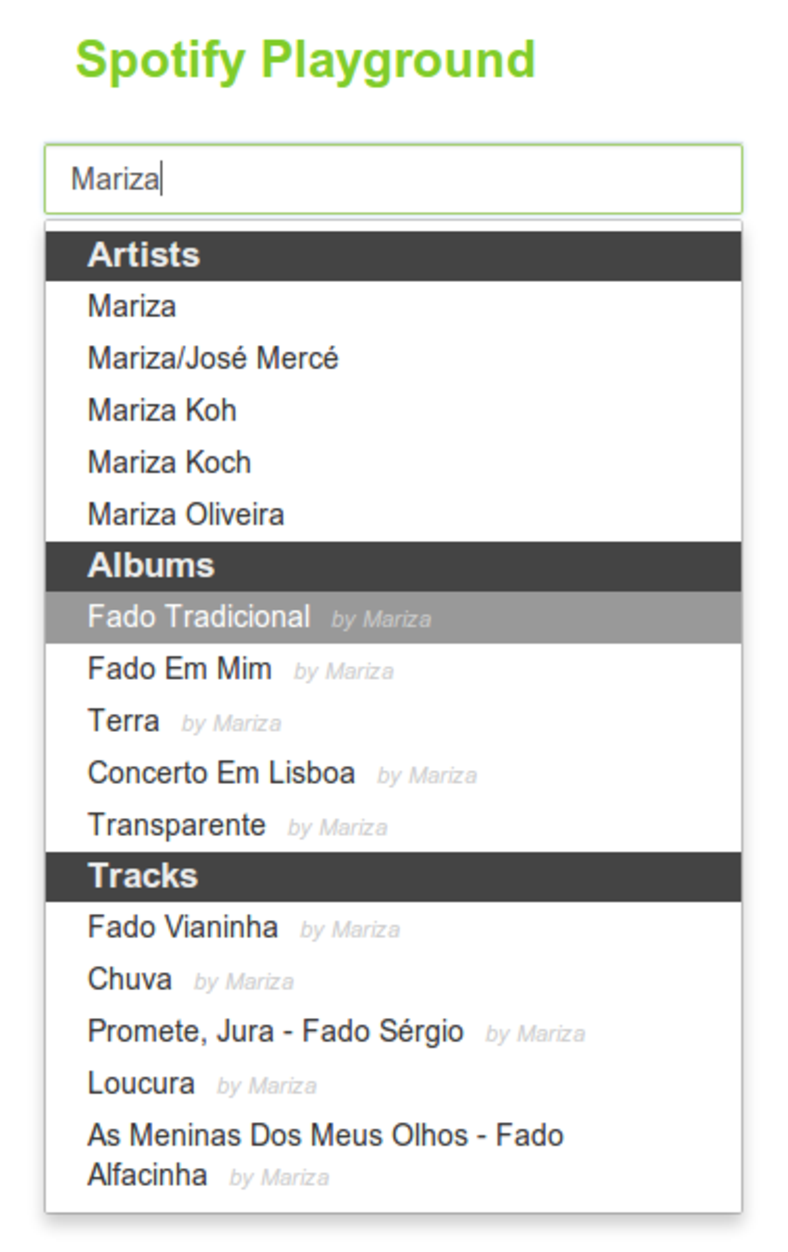
\includegraphics[width=\textwidth]{playground.pdf}
        \caption{Search result for "Mariza"}
        \label{fig:playgroun_a}
      \end{subfigure}

      \begin{subfigure}[b]{0.38\textwidth}
        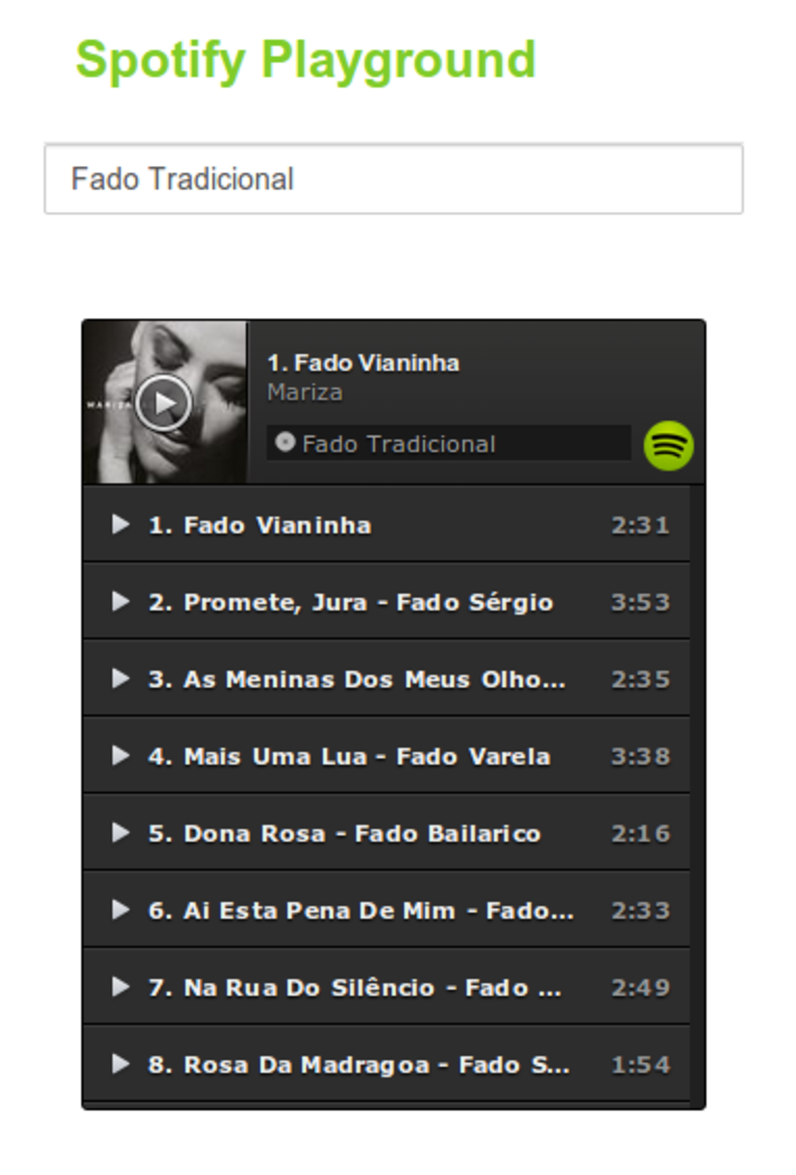
\includegraphics[width=\textwidth]{playground2.pdf}
        \caption{After selecting the album "Fado Tradicional" the \emph{Play button} displays all of the album's tracks to be played in sequence.}
        \label{fig:playground_b}
      \end{subfigure}

      \caption{Experiment with the \emph{Metadata API} and the \emph{Play Button Widget} (source code: \url{github.com/carsy/spotify-playground})}
      \label{fig:playground}

    \end{figure}

    Both tools turned out to be well documented and easy to use.


    Another experiment was made in order to assert the potential of Spotify Applications.
    There was a need to know if the canvas element was well supported by Spotify's environment, because that is the preferred way to graphically draw a graph.

    To test that, a simple application was created with the following code:

    \begin{lstlisting}[caption={\emph{iframe} element that allows to embed RAMA's website into the application.}, style=htmlcssjs]
      <iframe src="http://rama.inescporto.pt/app" frameborder="0">
      </iframe>\end{lstlisting}

    The final result can be seen in \ref{fig:rama_spotifyed}.

    \begin{figure}
      \begin{center}
        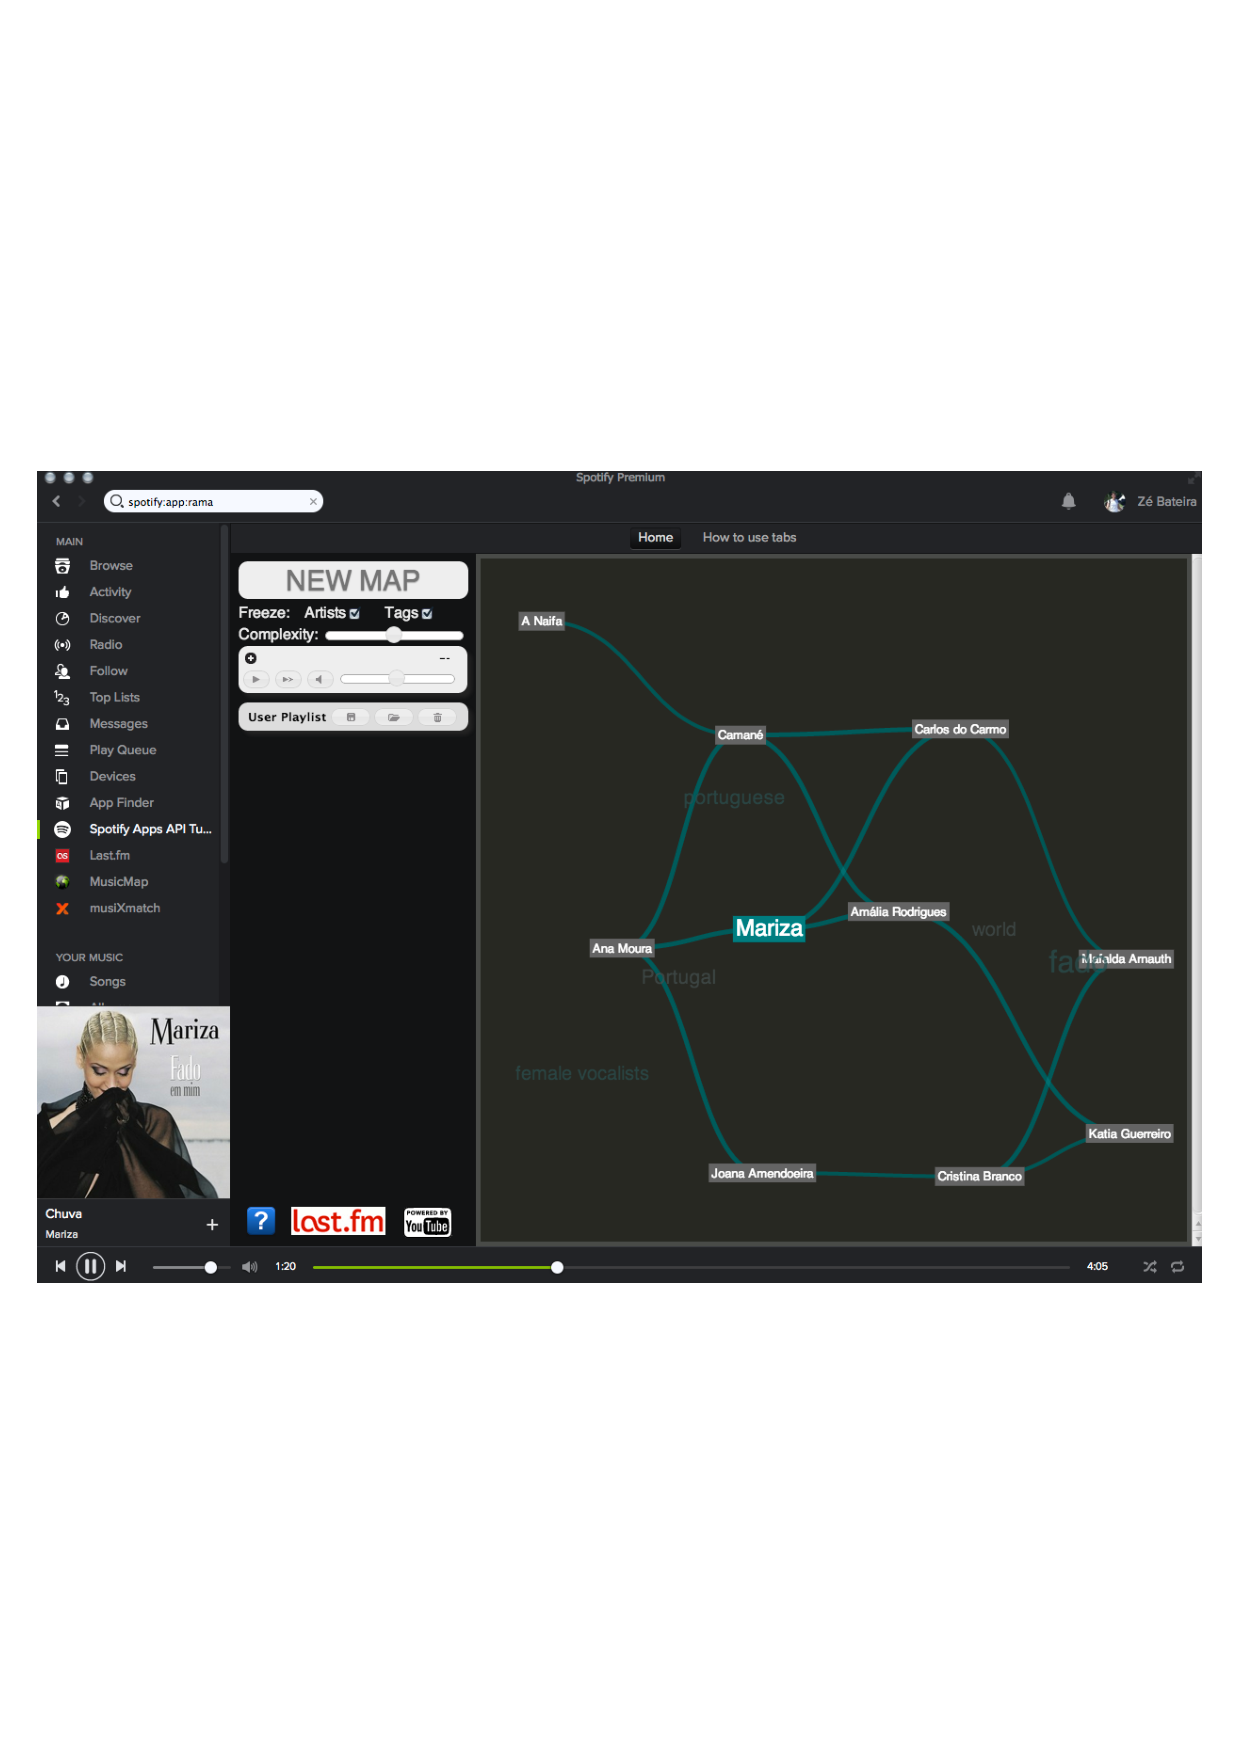
\includegraphics[width=\textwidth]{spotify_rama.embedded.pdf}
      \end{center}
      \caption{RAMA's website embedded into a Spotify Application.}
      \label{fig:rama_spotifyed}
    \end{figure}

    Although the \emph{iframe} and \emph{canvas} elements are supported, there are some that are not.
    This specific application is not usable since, for example, playing tracks from external sources is not allowed.

    Nonetheless, there is a way to test which Html elements are supported, using an internal Spotify application.
    In \ref{fig:canvas_support} one can see the 100\% supported canvas element.

    \begin{figure}
       \begin{center}
         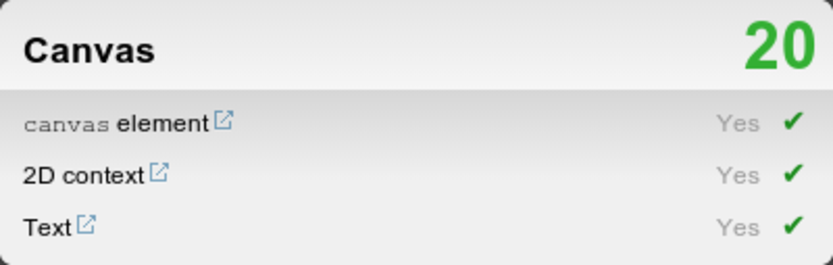
\includegraphics[width=0.5\textwidth]{canvas_support.pdf}
       \end{center}
       \caption{Test result for the canvas element.}
       \label{fig:canvas_support}
     \end{figure}

  % subsection experiments (end)

  \subsection{Conclusion} % (fold)
  \label{sub:conclusion}

    The developed prototype \ref{fig:rama_spotifyed} revealed to be the most appropriate to well integrate Spotify and RAMA.

    Given that, the proposed modules developed are \ref{item:obj4} and \ref{item:obj5}.

  % subsection conclusion (end)

% section spotify (end)

\section{Technologies used} % (fold)
\label{sec:technologies}

  The following technologies were used during the development of the application.

  \subsection{Spotify Desktop Client} % (fold)
  \label{sub:subsection_name}
    Spotify Applications are developed in its runtime environment - the Spotify Desktop Client.

    To open a Spotify Application, locally, one writes the following in the search bar: spotify:app:rama

    Where \emph{rama} is the application identifier declared in the \emph{manifest.json} file\footnote{file located at the root of the project folder}.

    Example:

    \lstinputlisting[caption={manifest.json: \emph{BundleIdentifier} is the application's identifier; \emph{Dependencies} declares the Application's API dependencies.}, style=htmlcssjs]{snippets/manifest.json}

    There are useful options for development located in the "Develop" tab (\ref{fig:html5_support}).
    The "Show Inspector" option opens the \emph{Webkit Development Tools} (\ref{sub:webkit_tools}) window.

    \begin{figure}[tb]
      \begin{center}
        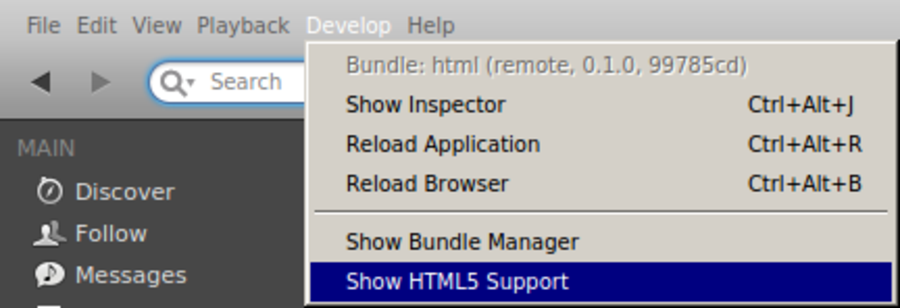
\includegraphics[width=\textwidth]{html5_support.pdf}
      \end{center}
      \caption{\emph{Develop} Tab}
      \label{fig:html5_support}
    \end{figure}
  
  \subsection{Webkit Development Tools - webkit.org} % (fold)
  \label{sub:webkit_tools}

    The webkit tools provides a bundle of tools for web development.

    \begin{figure}
      \begin{center}
        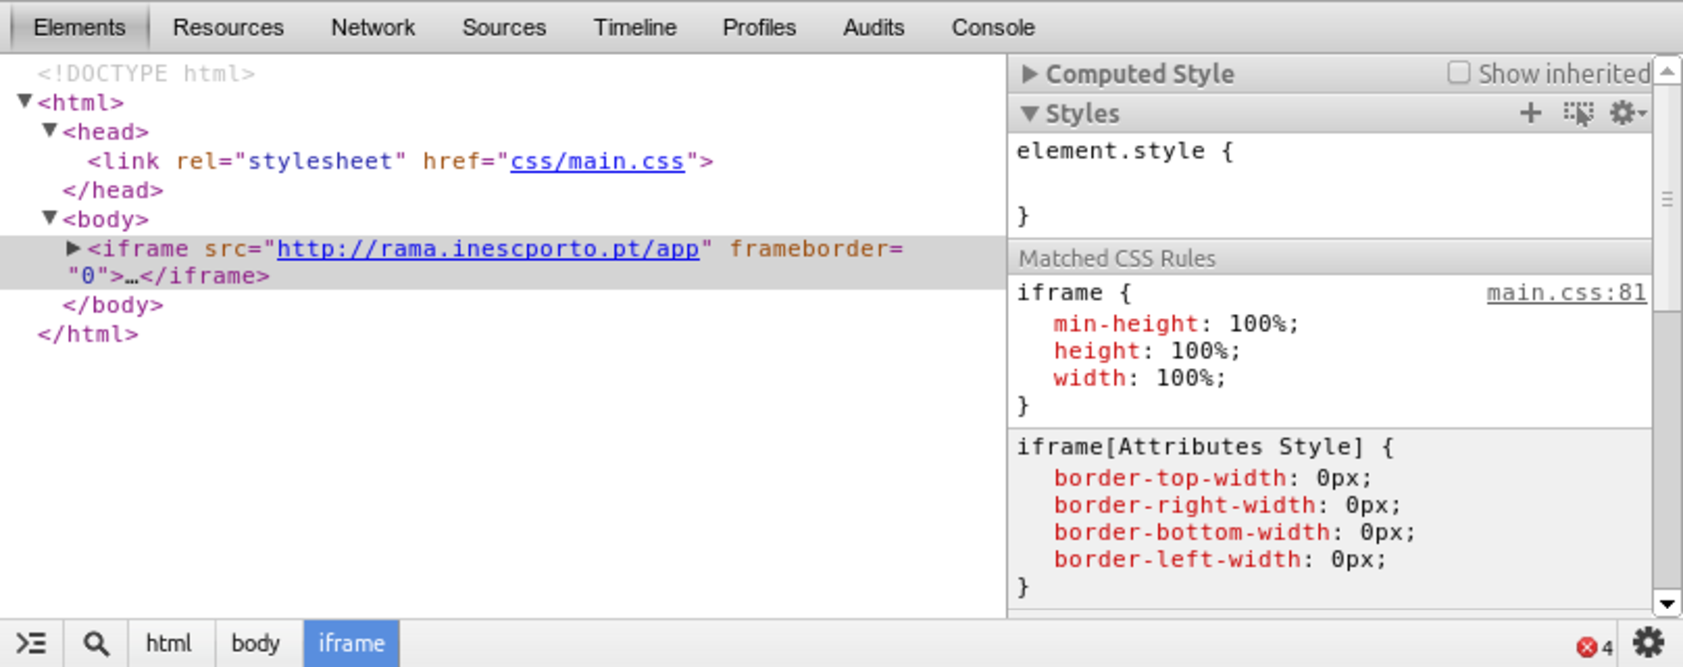
\includegraphics[width=\textwidth]{webkit_inspector.pdf}
      \end{center}
      \caption{Webkit: \emph{Inspector} tab view. Other tools available: \emph{Resources, Network, Sources, Timeline, Profiles, Audits} and \emph{Console}.}

      \label{fig:webkit_inspector}
    \end{figure}

    Being the most important:

    \begin{description}
      \item[Inspector] Allows to inspect the resulting Html and CSS and edit the code and see the application automatically reflect those changes (\ref{fig:webkit_inspector}).
      \item[Network] Shows a timeline list of resources that where loaded from external sources (sometimes local) (\ref{fig:webkit_network}).
      \item[Profile] Allows to identify which parts of the javascript code are being executed frequently, and which ones might be creating a performance issue (\ref{fig:webkit_profile}).
      \item[Audit] Helps to understand which CSS rules are not being used (\ref{fig:webkit_audit}).
      \item[Console] Javascript interpreter that also works as the log output for the application (\ref{fig:webkit_console}).

    \end{description}

    \begin{figure}
      \begin{center}
        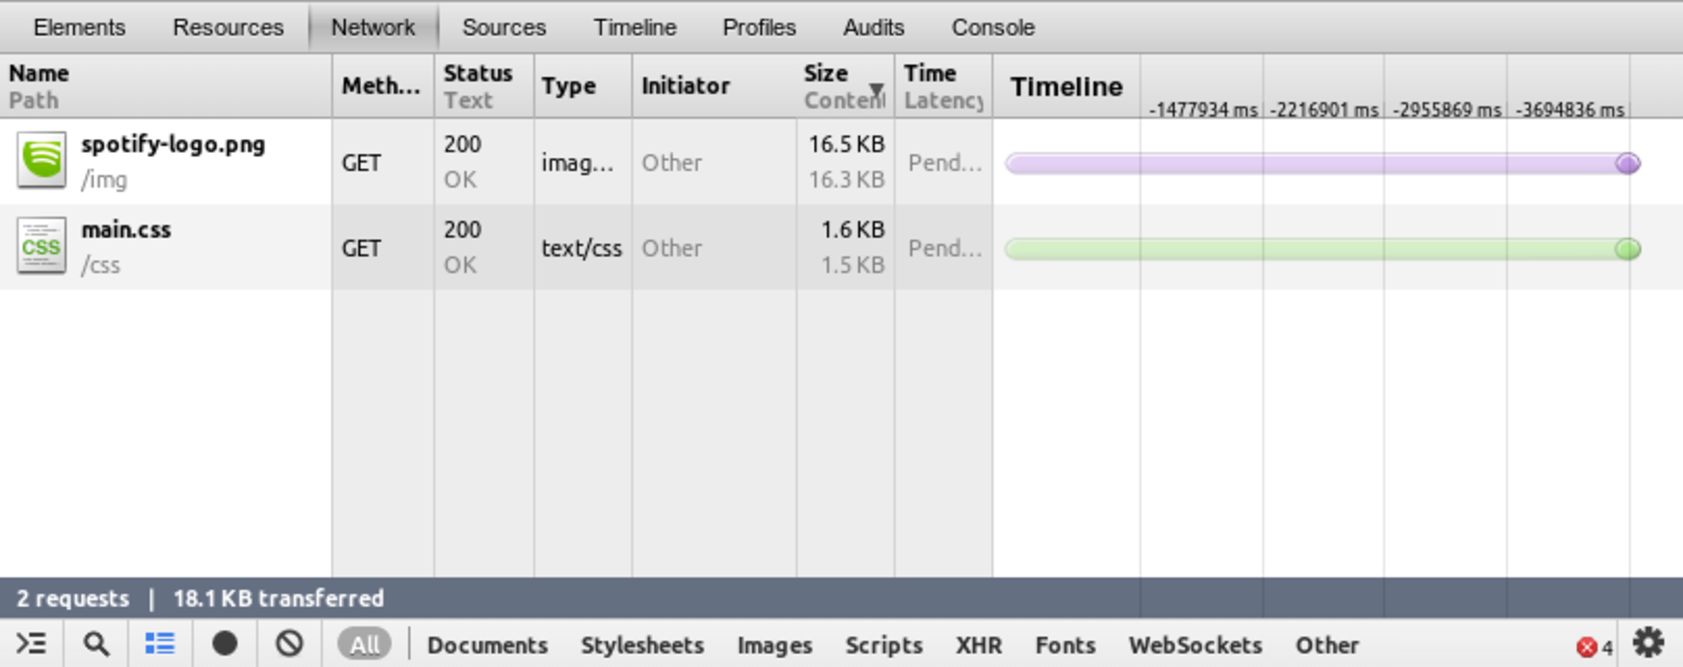
\includegraphics[width=\textwidth]{webkit_network.pdf}
      \end{center}
      \caption{Webkit Network}
      \label{fig:webkit_network}
    \end{figure}

    \begin{figure}
      \begin{center}
        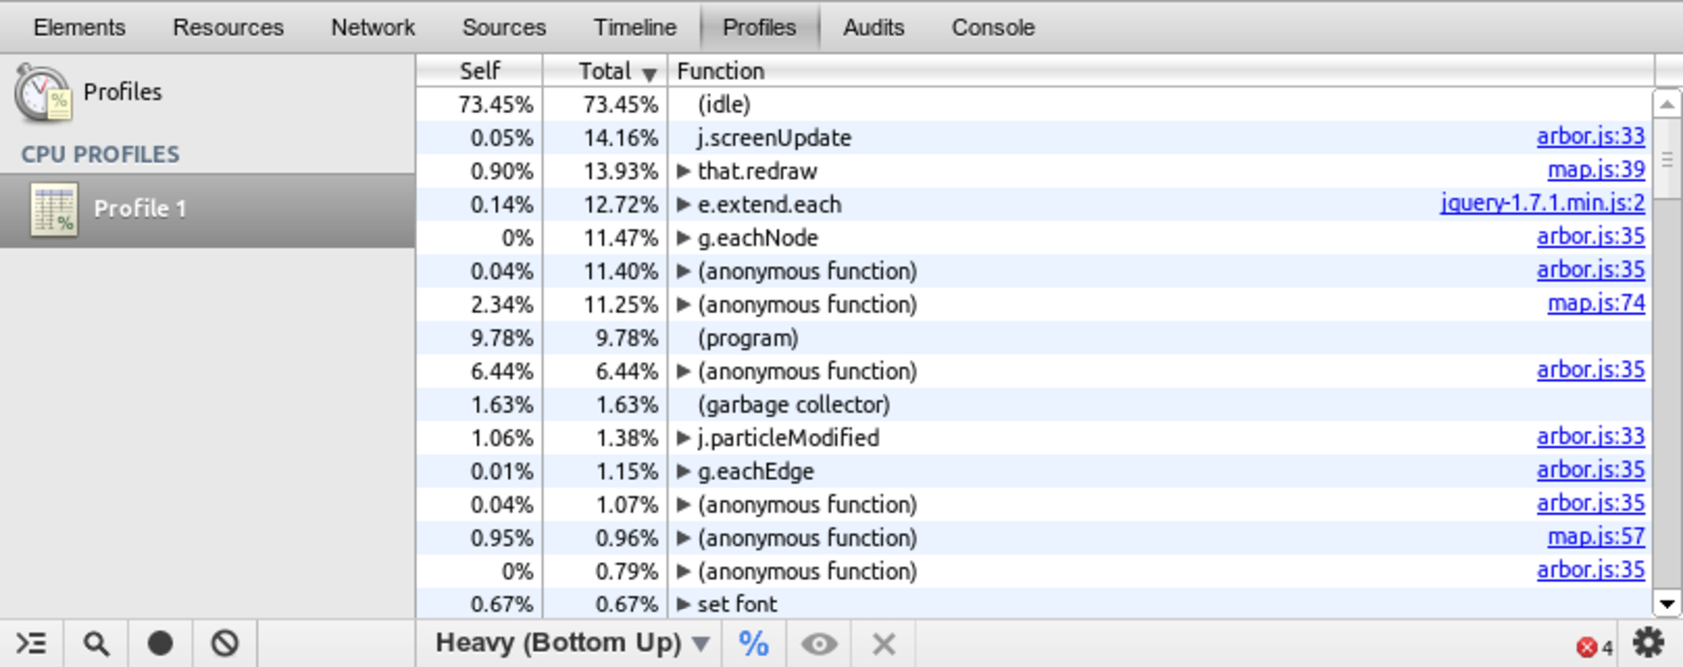
\includegraphics[width=\textwidth]{webkit_profile.pdf}
      \end{center}
      \caption{Webkit Profile: Canvas render functions are the ones taking up most of the processing cycles. However there is a JQuery function that used 12.75\% of processing time, which might indicate a performance issue to be improved.}
      \label{fig:webkit_profile}
    \end{figure}

    \begin{figure}
      \begin{center}
        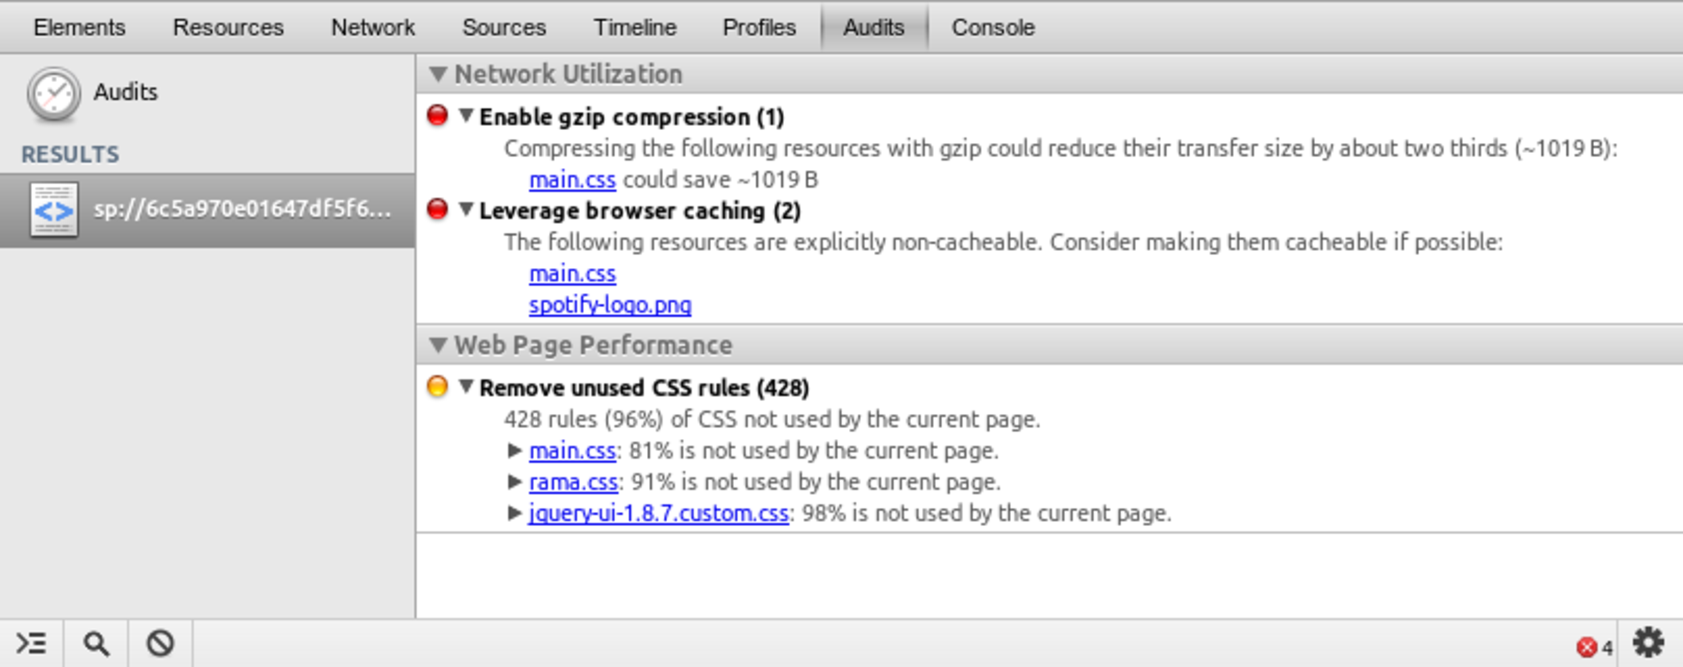
\includegraphics[width=\textwidth]{webkit_audit.pdf}
      \end{center}
      \caption{Webkit Audit: 96\% of the CSS code is not being used indicates a issue to be solved.}
      \label{fig:webkit_audit}
    \end{figure}

    \begin{figure}
      \begin{center}
        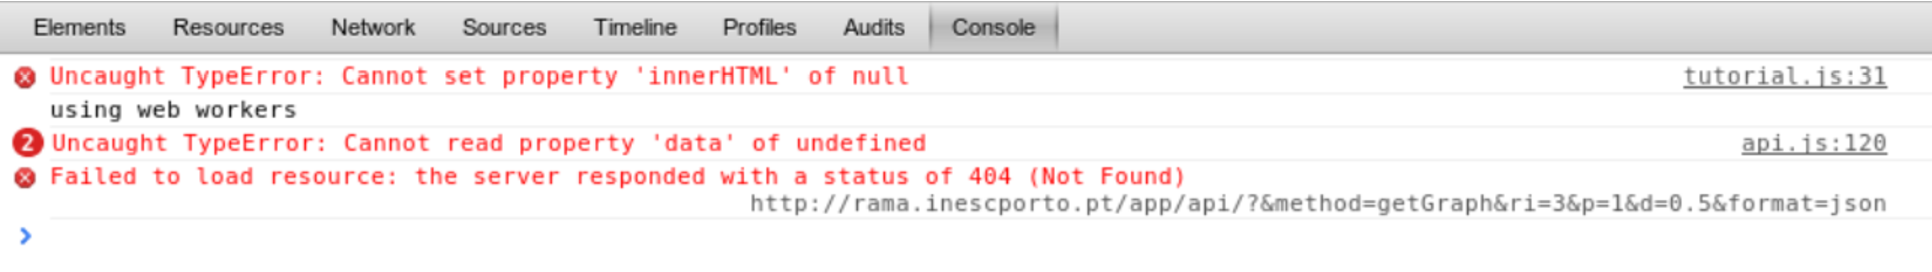
\includegraphics[width=\textwidth]{webkit_console.pdf}
      \end{center}
      \caption{Webkit Console: Javascript errors are reported there (and highlighted in red as well).}
      \label{fig:webkit_console}
    \end{figure}

  \subsection{Gruntjs - gruntjs.com} % (fold)
    \label{sub:gruntjs}
      Gruntjs is a Javascript task runner.
      It allows to automate most of the repetitive tasks when developing a website.
      Very useful for testing, compiling and code optimization.

  \subsection{Npmjs - npmjs.org} % (fold)
  \label{sub:npm}
    Package dependency manager for nodejs - Node Packaged Modules.
    Node packages will be used, since Gruntjs plugins are all nodejs packages (as well as Grunt itself).

    A npm configuration file (\emph{package.json}) allows to identify the packages that the application depends upon, as well as its versions.

    Example: 

    \lstinputlisting[caption={\emph{package.json}: "*" means that npm should always install the latest version of that package.}, style=htmlcssjs]{snippets/package.json}

  \subsection{Bower - bower.io} % (fold)
  \label{sub:bower}
  
  Bower is also a package manager, but oriented for web front-end packages.

  % subsection bower (end)

  \subsection{vis.js - visjs.org} % (fold)
  \label{sub:visjs}
    Javascript framework for visualization.
    It provides a few visual components, including graphs.

\section{Conclusions}

  The final choice is to develop the Spotify Application.

  Although the other proposals were also doable, the possibility to integrate a RAMA-like interface into Spotify's Desktop Client leaves a Spotify User more at ease with the environment.

  The prototype should implement the proposed modules \ref{item:obj4} and \ref{item:obj5}.